%! TEX program = xelatex
\documentclass{article} % For LaTeX2e
\usepackage{iclr2019_conference,times}

% Optional math commands from https://github.com/goodfeli/dlbook_notation.
%%%%% NEW MATH DEFINITIONS %%%%%

\usepackage{amsmath,amsfonts,bm}

% Mark sections of captions for referring to divisions of figures
\newcommand{\figleft}{{\em (Left)}}
\newcommand{\figcenter}{{\em (Center)}}
\newcommand{\figright}{{\em (Right)}}
\newcommand{\figtop}{{\em (Top)}}
\newcommand{\figbottom}{{\em (Bottom)}}
\newcommand{\captiona}{{\em (a)}}
\newcommand{\captionb}{{\em (b)}}
\newcommand{\captionc}{{\em (c)}}
\newcommand{\captiond}{{\em (d)}}

% Highlight a newly defined term
\newcommand{\newterm}[1]{{\bf #1}}


% Figure reference, lower-case.
\def\figref#1{figure~\ref{#1}}
% Figure reference, capital. For start of sentence
\def\Figref#1{Figure~\ref{#1}}
\def\twofigref#1#2{figures \ref{#1} and \ref{#2}}
\def\quadfigref#1#2#3#4{figures \ref{#1}, \ref{#2}, \ref{#3} and \ref{#4}}
% Section reference, lower-case.
\def\secref#1{section~\ref{#1}}
% Section reference, capital.
\def\Secref#1{Section~\ref{#1}}
% Reference to two sections.
\def\twosecrefs#1#2{sections \ref{#1} and \ref{#2}}
% Reference to three sections.
\def\secrefs#1#2#3{sections \ref{#1}, \ref{#2} and \ref{#3}}
% Reference to an equation, lower-case.
\def\eqref#1{equation~\ref{#1}}
% Reference to an equation, upper case
\def\Eqref#1{Equation~\ref{#1}}
% A raw reference to an equation---avoid using if possible
\def\plaineqref#1{\ref{#1}}
% Reference to a chapter, lower-case.
\def\chapref#1{chapter~\ref{#1}}
% Reference to an equation, upper case.
\def\Chapref#1{Chapter~\ref{#1}}
% Reference to a range of chapters
\def\rangechapref#1#2{chapters\ref{#1}--\ref{#2}}
% Reference to an algorithm, lower-case.
\def\algref#1{algorithm~\ref{#1}}
% Reference to an algorithm, upper case.
\def\Algref#1{Algorithm~\ref{#1}}
\def\twoalgref#1#2{algorithms \ref{#1} and \ref{#2}}
\def\Twoalgref#1#2{Algorithms \ref{#1} and \ref{#2}}
% Reference to a part, lower case
\def\partref#1{part~\ref{#1}}
% Reference to a part, upper case
\def\Partref#1{Part~\ref{#1}}
\def\twopartref#1#2{parts \ref{#1} and \ref{#2}}

\def\ceil#1{\lceil #1 \rceil}
\def\floor#1{\lfloor #1 \rfloor}
\def\1{\bm{1}}
\newcommand{\train}{\mathcal{D}}
\newcommand{\valid}{\mathcal{D_{\mathrm{valid}}}}
\newcommand{\test}{\mathcal{D_{\mathrm{test}}}}

\def\eps{{\epsilon}}


% Random variables
\def\reta{{\textnormal{$\eta$}}}
\def\ra{{\textnormal{a}}}
\def\rb{{\textnormal{b}}}
\def\rc{{\textnormal{c}}}
\def\rd{{\textnormal{d}}}
\def\re{{\textnormal{e}}}
\def\rf{{\textnormal{f}}}
\def\rg{{\textnormal{g}}}
\def\rh{{\textnormal{h}}}
\def\ri{{\textnormal{i}}}
\def\rj{{\textnormal{j}}}
\def\rk{{\textnormal{k}}}
\def\rl{{\textnormal{l}}}
% rm is already a command, just don't name any random variables m
\def\rn{{\textnormal{n}}}
\def\ro{{\textnormal{o}}}
\def\rp{{\textnormal{p}}}
\def\rq{{\textnormal{q}}}
\def\rr{{\textnormal{r}}}
\def\rs{{\textnormal{s}}}
\def\rt{{\textnormal{t}}}
\def\ru{{\textnormal{u}}}
\def\rv{{\textnormal{v}}}
\def\rw{{\textnormal{w}}}
\def\rx{{\textnormal{x}}}
\def\ry{{\textnormal{y}}}
\def\rz{{\textnormal{z}}}

% Random vectors
\def\rvepsilon{{\mathbf{\epsilon}}}
\def\rvtheta{{\mathbf{\theta}}}
\def\rva{{\mathbf{a}}}
\def\rvb{{\mathbf{b}}}
\def\rvc{{\mathbf{c}}}
\def\rvd{{\mathbf{d}}}
\def\rve{{\mathbf{e}}}
\def\rvf{{\mathbf{f}}}
\def\rvg{{\mathbf{g}}}
\def\rvh{{\mathbf{h}}}
\def\rvu{{\mathbf{i}}}
\def\rvj{{\mathbf{j}}}
\def\rvk{{\mathbf{k}}}
\def\rvl{{\mathbf{l}}}
\def\rvm{{\mathbf{m}}}
\def\rvn{{\mathbf{n}}}
\def\rvo{{\mathbf{o}}}
\def\rvp{{\mathbf{p}}}
\def\rvq{{\mathbf{q}}}
\def\rvr{{\mathbf{r}}}
\def\rvs{{\mathbf{s}}}
\def\rvt{{\mathbf{t}}}
\def\rvu{{\mathbf{u}}}
\def\rvv{{\mathbf{v}}}
\def\rvw{{\mathbf{w}}}
\def\rvx{{\mathbf{x}}}
\def\rvy{{\mathbf{y}}}
\def\rvz{{\mathbf{z}}}

% Elements of random vectors
\def\erva{{\textnormal{a}}}
\def\ervb{{\textnormal{b}}}
\def\ervc{{\textnormal{c}}}
\def\ervd{{\textnormal{d}}}
\def\erve{{\textnormal{e}}}
\def\ervf{{\textnormal{f}}}
\def\ervg{{\textnormal{g}}}
\def\ervh{{\textnormal{h}}}
\def\ervi{{\textnormal{i}}}
\def\ervj{{\textnormal{j}}}
\def\ervk{{\textnormal{k}}}
\def\ervl{{\textnormal{l}}}
\def\ervm{{\textnormal{m}}}
\def\ervn{{\textnormal{n}}}
\def\ervo{{\textnormal{o}}}
\def\ervp{{\textnormal{p}}}
\def\ervq{{\textnormal{q}}}
\def\ervr{{\textnormal{r}}}
\def\ervs{{\textnormal{s}}}
\def\ervt{{\textnormal{t}}}
\def\ervu{{\textnormal{u}}}
\def\ervv{{\textnormal{v}}}
\def\ervw{{\textnormal{w}}}
\def\ervx{{\textnormal{x}}}
\def\ervy{{\textnormal{y}}}
\def\ervz{{\textnormal{z}}}

% Random matrices
\def\rmA{{\mathbf{A}}}
\def\rmB{{\mathbf{B}}}
\def\rmC{{\mathbf{C}}}
\def\rmD{{\mathbf{D}}}
\def\rmE{{\mathbf{E}}}
\def\rmF{{\mathbf{F}}}
\def\rmG{{\mathbf{G}}}
\def\rmH{{\mathbf{H}}}
\def\rmI{{\mathbf{I}}}
\def\rmJ{{\mathbf{J}}}
\def\rmK{{\mathbf{K}}}
\def\rmL{{\mathbf{L}}}
\def\rmM{{\mathbf{M}}}
\def\rmN{{\mathbf{N}}}
\def\rmO{{\mathbf{O}}}
\def\rmP{{\mathbf{P}}}
\def\rmQ{{\mathbf{Q}}}
\def\rmR{{\mathbf{R}}}
\def\rmS{{\mathbf{S}}}
\def\rmT{{\mathbf{T}}}
\def\rmU{{\mathbf{U}}}
\def\rmV{{\mathbf{V}}}
\def\rmW{{\mathbf{W}}}
\def\rmX{{\mathbf{X}}}
\def\rmY{{\mathbf{Y}}}
\def\rmZ{{\mathbf{Z}}}

% Elements of random matrices
\def\ermA{{\textnormal{A}}}
\def\ermB{{\textnormal{B}}}
\def\ermC{{\textnormal{C}}}
\def\ermD{{\textnormal{D}}}
\def\ermE{{\textnormal{E}}}
\def\ermF{{\textnormal{F}}}
\def\ermG{{\textnormal{G}}}
\def\ermH{{\textnormal{H}}}
\def\ermI{{\textnormal{I}}}
\def\ermJ{{\textnormal{J}}}
\def\ermK{{\textnormal{K}}}
\def\ermL{{\textnormal{L}}}
\def\ermM{{\textnormal{M}}}
\def\ermN{{\textnormal{N}}}
\def\ermO{{\textnormal{O}}}
\def\ermP{{\textnormal{P}}}
\def\ermQ{{\textnormal{Q}}}
\def\ermR{{\textnormal{R}}}
\def\ermS{{\textnormal{S}}}
\def\ermT{{\textnormal{T}}}
\def\ermU{{\textnormal{U}}}
\def\ermV{{\textnormal{V}}}
\def\ermW{{\textnormal{W}}}
\def\ermX{{\textnormal{X}}}
\def\ermY{{\textnormal{Y}}}
\def\ermZ{{\textnormal{Z}}}

% Vectors
\def\vzero{{\bm{0}}}
\def\vone{{\bm{1}}}
\def\vmu{{\bm{\mu}}}
\def\vtheta{{\bm{\theta}}}
\def\va{{\bm{a}}}
\def\vb{{\bm{b}}}
\def\vc{{\bm{c}}}
\def\vd{{\bm{d}}}
\def\ve{{\bm{e}}}
\def\vf{{\bm{f}}}
\def\vg{{\bm{g}}}
\def\vh{{\bm{h}}}
\def\vi{{\bm{i}}}
\def\vj{{\bm{j}}}
\def\vk{{\bm{k}}}
\def\vl{{\bm{l}}}
\def\vm{{\bm{m}}}
\def\vn{{\bm{n}}}
\def\vo{{\bm{o}}}
\def\vp{{\bm{p}}}
\def\vq{{\bm{q}}}
\def\vr{{\bm{r}}}
\def\vs{{\bm{s}}}
\def\vt{{\bm{t}}}
\def\vu{{\bm{u}}}
\def\vv{{\bm{v}}}
\def\vw{{\bm{w}}}
\def\vx{{\bm{x}}}
\def\vy{{\bm{y}}}
\def\vz{{\bm{z}}}

% Elements of vectors
\def\evalpha{{\alpha}}
\def\evbeta{{\beta}}
\def\evepsilon{{\epsilon}}
\def\evlambda{{\lambda}}
\def\evomega{{\omega}}
\def\evmu{{\mu}}
\def\evpsi{{\psi}}
\def\evsigma{{\sigma}}
\def\evtheta{{\theta}}
\def\eva{{a}}
\def\evb{{b}}
\def\evc{{c}}
\def\evd{{d}}
\def\eve{{e}}
\def\evf{{f}}
\def\evg{{g}}
\def\evh{{h}}
\def\evi{{i}}
\def\evj{{j}}
\def\evk{{k}}
\def\evl{{l}}
\def\evm{{m}}
\def\evn{{n}}
\def\evo{{o}}
\def\evp{{p}}
\def\evq{{q}}
\def\evr{{r}}
\def\evs{{s}}
\def\evt{{t}}
\def\evu{{u}}
\def\evv{{v}}
\def\evw{{w}}
\def\evx{{x}}
\def\evy{{y}}
\def\evz{{z}}

% Matrix
\def\mA{{\bm{A}}}
\def\mB{{\bm{B}}}
\def\mC{{\bm{C}}}
\def\mD{{\bm{D}}}
\def\mE{{\bm{E}}}
\def\mF{{\bm{F}}}
\def\mG{{\bm{G}}}
\def\mH{{\bm{H}}}
\def\mI{{\bm{I}}}
\def\mJ{{\bm{J}}}
\def\mK{{\bm{K}}}
\def\mL{{\bm{L}}}
\def\mM{{\bm{M}}}
\def\mN{{\bm{N}}}
\def\mO{{\bm{O}}}
\def\mP{{\bm{P}}}
\def\mQ{{\bm{Q}}}
\def\mR{{\bm{R}}}
\def\mS{{\bm{S}}}
\def\mT{{\bm{T}}}
\def\mU{{\bm{U}}}
\def\mV{{\bm{V}}}
\def\mW{{\bm{W}}}
\def\mX{{\bm{X}}}
\def\mY{{\bm{Y}}}
\def\mZ{{\bm{Z}}}
\def\mBeta{{\bm{\beta}}}
\def\mPhi{{\bm{\Phi}}}
\def\mLambda{{\bm{\Lambda}}}
\def\mSigma{{\bm{\Sigma}}}

% Tensor
\DeclareMathAlphabet{\mathsfit}{\encodingdefault}{\sfdefault}{m}{sl}
\SetMathAlphabet{\mathsfit}{bold}{\encodingdefault}{\sfdefault}{bx}{n}
\newcommand{\tens}[1]{\bm{\mathsfit{#1}}}
\def\tA{{\tens{A}}}
\def\tB{{\tens{B}}}
\def\tC{{\tens{C}}}
\def\tD{{\tens{D}}}
\def\tE{{\tens{E}}}
\def\tF{{\tens{F}}}
\def\tG{{\tens{G}}}
\def\tH{{\tens{H}}}
\def\tI{{\tens{I}}}
\def\tJ{{\tens{J}}}
\def\tK{{\tens{K}}}
\def\tL{{\tens{L}}}
\def\tM{{\tens{M}}}
\def\tN{{\tens{N}}}
\def\tO{{\tens{O}}}
\def\tP{{\tens{P}}}
\def\tQ{{\tens{Q}}}
\def\tR{{\tens{R}}}
\def\tS{{\tens{S}}}
\def\tT{{\tens{T}}}
\def\tU{{\tens{U}}}
\def\tV{{\tens{V}}}
\def\tW{{\tens{W}}}
\def\tX{{\tens{X}}}
\def\tY{{\tens{Y}}}
\def\tZ{{\tens{Z}}}


% Graph
\def\gA{{\mathcal{A}}}
\def\gB{{\mathcal{B}}}
\def\gC{{\mathcal{C}}}
\def\gD{{\mathcal{D}}}
\def\gE{{\mathcal{E}}}
\def\gF{{\mathcal{F}}}
\def\gG{{\mathcal{G}}}
\def\gH{{\mathcal{H}}}
\def\gI{{\mathcal{I}}}
\def\gJ{{\mathcal{J}}}
\def\gK{{\mathcal{K}}}
\def\gL{{\mathcal{L}}}
\def\gM{{\mathcal{M}}}
\def\gN{{\mathcal{N}}}
\def\gO{{\mathcal{O}}}
\def\gP{{\mathcal{P}}}
\def\gQ{{\mathcal{Q}}}
\def\gR{{\mathcal{R}}}
\def\gS{{\mathcal{S}}}
\def\gT{{\mathcal{T}}}
\def\gU{{\mathcal{U}}}
\def\gV{{\mathcal{V}}}
\def\gW{{\mathcal{W}}}
\def\gX{{\mathcal{X}}}
\def\gY{{\mathcal{Y}}}
\def\gZ{{\mathcal{Z}}}

% Sets
\def\sA{{\mathbb{A}}}
\def\sB{{\mathbb{B}}}
\def\sC{{\mathbb{C}}}
\def\sD{{\mathbb{D}}}
% Don't use a set called E, because this would be the same as our symbol
% for expectation.
\def\sF{{\mathbb{F}}}
\def\sG{{\mathbb{G}}}
\def\sH{{\mathbb{H}}}
\def\sI{{\mathbb{I}}}
\def\sJ{{\mathbb{J}}}
\def\sK{{\mathbb{K}}}
\def\sL{{\mathbb{L}}}
\def\sM{{\mathbb{M}}}
\def\sN{{\mathbb{N}}}
\def\sO{{\mathbb{O}}}
\def\sP{{\mathbb{P}}}
\def\sQ{{\mathbb{Q}}}
\def\sR{{\mathbb{R}}}
\def\sS{{\mathbb{S}}}
\def\sT{{\mathbb{T}}}
\def\sU{{\mathbb{U}}}
\def\sV{{\mathbb{V}}}
\def\sW{{\mathbb{W}}}
\def\sX{{\mathbb{X}}}
\def\sY{{\mathbb{Y}}}
\def\sZ{{\mathbb{Z}}}

% Entries of a matrix
\def\emLambda{{\Lambda}}
\def\emA{{A}}
\def\emB{{B}}
\def\emC{{C}}
\def\emD{{D}}
\def\emE{{E}}
\def\emF{{F}}
\def\emG{{G}}
\def\emH{{H}}
\def\emI{{I}}
\def\emJ{{J}}
\def\emK{{K}}
\def\emL{{L}}
\def\emM{{M}}
\def\emN{{N}}
\def\emO{{O}}
\def\emP{{P}}
\def\emQ{{Q}}
\def\emR{{R}}
\def\emS{{S}}
\def\emT{{T}}
\def\emU{{U}}
\def\emV{{V}}
\def\emW{{W}}
\def\emX{{X}}
\def\emY{{Y}}
\def\emZ{{Z}}
\def\emSigma{{\Sigma}}

% entries of a tensor
% Same font as tensor, without \bm wrapper
\newcommand{\etens}[1]{\mathsfit{#1}}
\def\etLambda{{\etens{\Lambda}}}
\def\etA{{\etens{A}}}
\def\etB{{\etens{B}}}
\def\etC{{\etens{C}}}
\def\etD{{\etens{D}}}
\def\etE{{\etens{E}}}
\def\etF{{\etens{F}}}
\def\etG{{\etens{G}}}
\def\etH{{\etens{H}}}
\def\etI{{\etens{I}}}
\def\etJ{{\etens{J}}}
\def\etK{{\etens{K}}}
\def\etL{{\etens{L}}}
\def\etM{{\etens{M}}}
\def\etN{{\etens{N}}}
\def\etO{{\etens{O}}}
\def\etP{{\etens{P}}}
\def\etQ{{\etens{Q}}}
\def\etR{{\etens{R}}}
\def\etS{{\etens{S}}}
\def\etT{{\etens{T}}}
\def\etU{{\etens{U}}}
\def\etV{{\etens{V}}}
\def\etW{{\etens{W}}}
\def\etX{{\etens{X}}}
\def\etY{{\etens{Y}}}
\def\etZ{{\etens{Z}}}

% The true underlying data generating distribution
\newcommand{\pdata}{p_{\rm{data}}}
% The empirical distribution defined by the training set
\newcommand{\ptrain}{\hat{p}_{\rm{data}}}
\newcommand{\Ptrain}{\hat{P}_{\rm{data}}}
% The model distribution
\newcommand{\pmodel}{p_{\rm{model}}}
\newcommand{\Pmodel}{P_{\rm{model}}}
\newcommand{\ptildemodel}{\tilde{p}_{\rm{model}}}
% Stochastic autoencoder distributions
\newcommand{\pencode}{p_{\rm{encoder}}}
\newcommand{\pdecode}{p_{\rm{decoder}}}
\newcommand{\precons}{p_{\rm{reconstruct}}}

\newcommand{\laplace}{\mathrm{Laplace}} % Laplace distribution

\newcommand{\E}{\mathbb{E}}
\newcommand{\Ls}{\mathcal{L}}
\newcommand{\R}{\mathbb{R}}
\newcommand{\emp}{\tilde{p}}
\newcommand{\lr}{\alpha}
\newcommand{\reg}{\lambda}
\newcommand{\rect}{\mathrm{rectifier}}
\newcommand{\softmax}{\mathrm{softmax}}
\newcommand{\sigmoid}{\sigma}
\newcommand{\softplus}{\zeta}
\newcommand{\KL}{D_{\mathrm{KL}}}
\newcommand{\Var}{\mathrm{Var}}
\newcommand{\standarderror}{\mathrm{SE}}
\newcommand{\Cov}{\mathrm{Cov}}
% Wolfram Mathworld says $L^2$ is for function spaces and $\ell^2$ is for vectors
% But then they seem to use $L^2$ for vectors throughout the site, and so does
% wikipedia.
\newcommand{\normlzero}{L^0}
\newcommand{\normlone}{L^1}
\newcommand{\normltwo}{L^2}
\newcommand{\normlp}{L^p}
\newcommand{\normmax}{L^\infty}

\newcommand{\parents}{Pa} % See usage in notation.tex. Chosen to match Daphne's book.

\DeclareMathOperator*{\argmax}{arg\,max}
\DeclareMathOperator*{\argmin}{arg\,min}

\DeclareMathOperator{\sign}{sign}
\DeclareMathOperator{\Tr}{Tr}
\let\ab\allowbreak


\usepackage{hyperref}
\usepackage{url}

\usepackage{graphicx,caption,subfig}
\graphicspath{
  {figures/}
}
\usepackage{amsmath,bm}
\newcommand{\norm}[1]{\left\lVert#1\right\rVert}

\title{EE236C Project Report:\\Video Stabilization}

% Authors must not appear in the submitted version. They should be hidden
% as long as the \iclrfinalcopy macro remains commented out below.
% Non-anonymous submissions will be rejected without review.

\author{Ryan Neph \\
Department of Radiation Oncology \\
UCLA Physics and Biology in Medicine \\
Los Angeles, CA 90095, USA \\
\texttt{ryanneph@ucla.edu} \\
}

% The \author macro works with any number of authors. There are two commands
% used to separate the names and addresses of multiple authors: \And and \AND.
%
% Using \And between authors leaves it to \LaTeX{} to determine where to break
% the lines. Using \AND forces a linebreak at that point. So, if \LaTeX{}
% puts 3 of 4 authors names on the first line, and the last on the second
% line, try using \AND instead of \And before the third author name.

\newcommand{\fix}{\marginpar{FIX}}
\newcommand{\new}{\marginpar{NEW}}

\iclrfinalcopy % Uncomment for camera-ready version, but NOT for submission.
\begin{document}


\maketitle

% \begin{abstract}
%   ABSTRACT TEXT
% \end{abstract}

\section{Introduction}
Video media is increasingly becoming one of the most popular ways to share stories between people. Once reserved for professionals, the ubiquity of software assisted imaging systems such as those found in nearly every smartphone, has opened the door for amateur filmmakers and non-filmmakers alike to approach a polished quality of video recording. One obvious difficulty associated with video recording in hand-held situations is controlling the camera to produce the intended effect for the viewer. In many cases, this intended effect is simply to reduce unintended motion induced by shakiness and jitter, while keeping the camera's gaze on some subject of interest. Various camera mounting systems have been used to this effect, including the simple tripod to remove all translational motion, the dolly, crane, and slider, to limit the motion to smooth realizations, often constrained by the mechanical limits of the system, and even mobile Steady-Cam rigs and self-correcting gimbals, which attempt to smooth unconstrained motion for more dynamic shots. The problems with each of these solutions lie in the cost and inconvenience of storing, transporting, and configuring this equipment, that generally limits their applicability to all except large commercial productions.

Instead, particularly in the last decade, great focus has been placed on software stabilization of video software assisted imaging systems such as those found in nearly every smartphone. This technology has opened the door for low- or no-budget "productions" to approach a polished quality of video presentation with minimal effort. Though, this technology has advanced significantly since its development, it is still limited in terms of its processing speed, and ability to produce the desired results in all situations, for all types of video. Of primary concern is the ability to meet the demands of video stability amidst the increasing resolution and frame-rate preferred by content creators. For example, in the last 5 years, the demand for 4K and 60 frames-per-second (fps) video has increased, carrying with it a substantial increase in the amount of data that must be processed before publishing each video. To meet these demands, while still providing a pleasing stabilization result, large-scale optimization methods, that are designed to handle large problem-scales are critical.



\section{Methods}
The approach taken to achieve stabilization of a video sequence consists of the following three main steps: 1) estimation of camera motion, 2) determination of smoothed camera motion, 3) reconstruction of stabilized video from smoothed motion. Each of these steps will be explained in the subsequent sections.

\subsection{Estimating Camera Motion}
Estimation of the camera's motion trajectory can be obtained either in 2D or 3D, using one of many methods that first impose a motion model on the camera's behaviour, then fit that model for each video frame based on a dense optical flow between frames, or more commonly a sparse feature correspondence. In this work, the latter approach is taken for efficiency, by first computing a sparse set of salient image features using a corner detector (Good Features To Track; GFTT) developed by \cite{JianboShi1994}; other options such as SIFT (\cite{Lowe2004}), SURF (\cite{Bay2006}), and FAST (\cite{Rosten2006}) are also used frequently to similar effect.

In particular, GFTT is used to select a set of up to 30 of the most prominent salient points, $p^{(i)}$, in each frame $F^{(i)}$ for $i=1,\dotsc,N-1$ (shown in figure \ref{fig:trackedfeatures}). Next, a correspondence of tracking points $(p^{(i)}, \hat{p}^{(i+1)})$ is fit for each pair of frames $(F^{(i)}, F^{(i+1)})$, using the sparse, image pyramid-based, optical flow method, developed by \cite{Lucas1981}. From this correspondence, the GFTT-detected points for frame $F^{(i)}$ are identified in frame $F^{(i+1)}$, excluding those that cannot be reliably located. Using the correspondence, a 2D affine mapping, $A^{(i)}$, is calculated for each frame pair, such that $\hat{p}^{(i+1)}_k = A^{(i)} p^{(i)}_k$, for each of the $k$ corresponding points.

\begin{figure}[h]
  \subfloat{{ 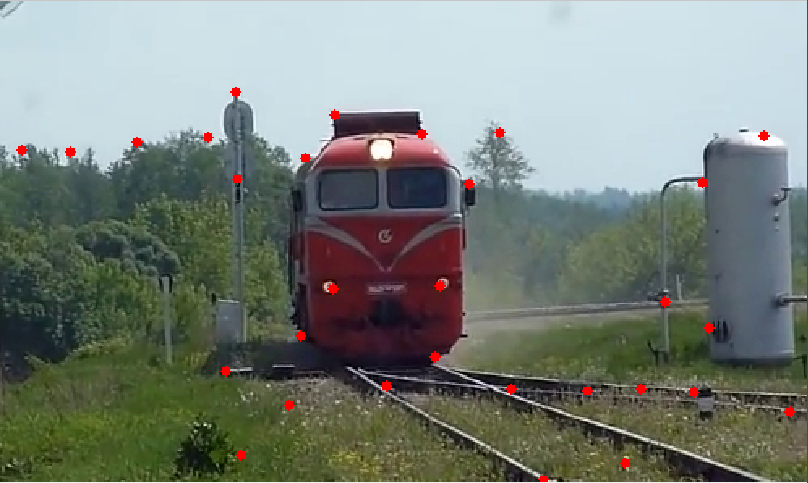
\includegraphics[width=0.5\textwidth]{tracked_features.png} }}
  \subfloat{{ 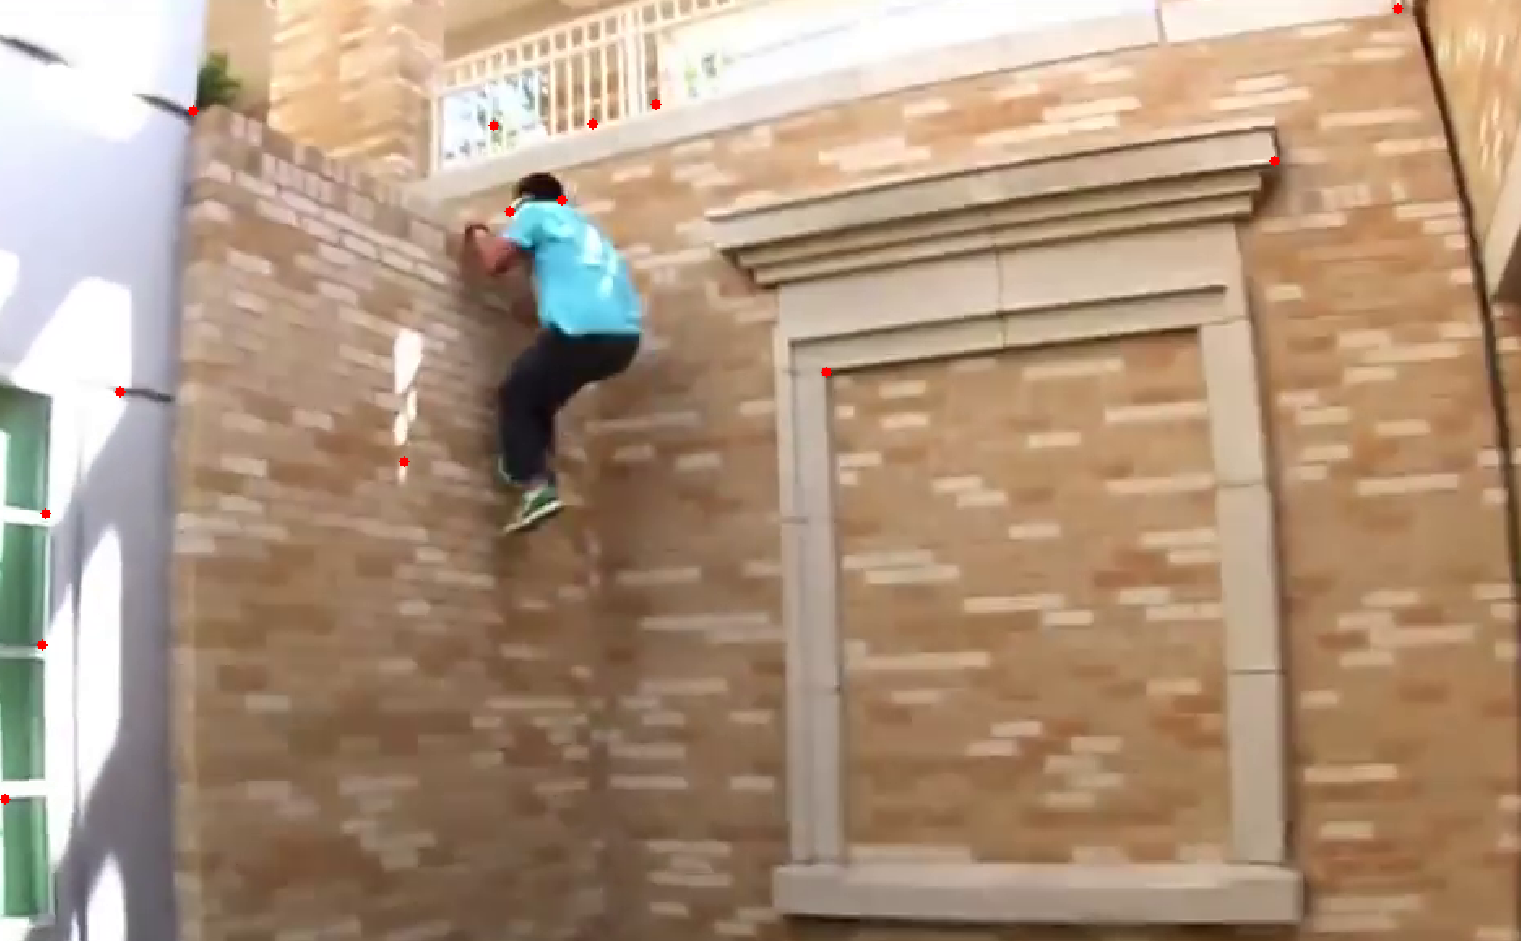
\includegraphics[width=0.5\textwidth]{tracked_features2.png} }}
  \caption{Original video frames with tracking points identified (red dots)}
  \label{fig:trackedfeatures}
\end{figure}

Once the sequence of 2D affine mapping matrices has been obtained, it is decomposed into 5 independent temporal parameter vectors for scale ($x$ and $y$ direction), rotation, and translation ($x$ and $y$): $s_x, s_y, r, t_x, t_y \in \mathbb{R}^N-1$. Motion trajectories for each degree of freedom are generated by computing the cumulative product ($s_x and s_y$), and cumulative sum ($r, t_x, and t_y$).

\subsection{Trajectory Smoothing with Huber-Regularized Temporal Finite Differences}
The basic formulation used in this work to achieve temporal video stabilization consists of a trajectory fidelity term to preserve the intent of the original video sequence, and a trajectory smoothness term to remove undesirable shaking and jittering. The former is defined as an $L_2$ error on the temporal camera motion for each degree of freedom (DOF), and the latter as an $L_1$ penalization of differences in first and second order forward differences of adjacent frames. The 1-norm is selected in this model to promote sparsity of the differences, encouraging piecewise smoothness in the first and second order derivatives of each DOF. To make this problem solvable by efficient methods, the 1-norm is relaxed by Moreau-Yosida smoothing to the smooth Huber penalty with parameter $\mu$ specifying the strength of the relaxation. The objective function on each DOF is:
\begin{equation*}
  G(\nu) = \norm{\nu - \hat{\nu}}_2^2 + \lambda_1 \norm{D \nu}_1^{(\mu)} + \lambda_2 \norm{D^2 \nu}_1^{(\mu)},
\end{equation*}
giving rise to the convex optimization problem:
\begin{align} \label{eq:optprob}
  & \underset{s_x, s_y, r, t_x, t_y}{\text{minimize}} & & G(s_x) + G(s_y) + G(r) + G(t_x) + G(t_y) \\
  & \text{subject to} & & s_{min} \le s_x^{(i)} \le s_{max}  \qquad{} \text{for }i=1,\dotsc,N \nonumber \\
  &                   & & s_{min} \le s_y^{(i)} \le s_{max} \nonumber \\
  &                   & & r_{min} \le r^{(i)}   \le r_{max} \nonumber \\
  &                   & & t_{min} \le t_x^{(i)} \le t_{max} \nonumber \\
  &                   & & t_{min} \le t_y^{(i)} \le t_{max} \nonumber
\end{align}
$\hat{\nu}\in \mathbb{R}^N$ is the unstabilized motion of one degree of freedom for $N$ video frames, $D$ and $D^2$ are the first and second order forward differencing operators, respectively, and $\norm{\cdot}_1^{(\mu)}$ is the Huber function defined as:
\begin{equation*}
  \norm{x}_1^{(\mu)} = \sum_{i=1}^N{\phi({x})},
\end{equation*}
with,
\begin{equation*}
  \phi(x)_i =
  \begin{cases}
    x^2/(2t)  & |x| \le \mu \\
   |z| - t/2  & |x| \ge \mu
  \end{cases}.
\end{equation*}

The parameters $\lambda$ and $\mu$ can be adjusted for each DOF to trade-off motion fidelity, smoothness, and optimization difficulty as desired. Increasing $\lambda$ will place a greater bias on smooth motion instead of original motion. Decreasing $\mu$ will result in a better approximation to the 1-norm, eliminating more small camera jitter, at the cost of increased optimization difficulty.

To solve the constrained convex optimization problem in (\ref{eq:optprob}), the Fast Iterative Shrinkage and Thresholding (FISTA) algorithm (\cite{Beck2009}) was used. FISTA solves problems of the form:
\begin{equation*}
  \underset{x}{\text{minimize}} \qquad{} F(x) + H(x)
\end{equation*}
$F(x)$ is assumed to have an $L$-Lipschitz gradient, and $H(x)$ is convex, but non-smooth, with a simple proximal operator. Adapting the convex minimization problem in (\ref{eq:optprob}), we get the equivalent problem:
\begin{align} \label{eq:optprob2}
  & \underset{s_x, s_y, r, t_x, t_y}{\text{minimize}} & & G(s_x) + G(s_y) + G(r) + G(t_x) + G(t_y) + {} \\
  & & & \delta_{Box[s_{min}, s_{max}]}(s_x) + \delta_{Box[s_{min}, s_{max}]}(s_y) + {} \nonumber \\
  & & & \delta_{Box[r_{min}, r_{max}]}(r) + {} \nonumber \\
  & & & \delta_{Box[t_{min}, t_{max}]}(t_x) + \delta_{Box[t_{min}, t_{max}]}(t_y), \nonumber
\end{align}
where the sum of indicator functions for the box constraints make up the non-smooth function $H(x)$, and the sum of each $G(x)$ applied to the 5 DOF vectors makes up the differentiable function $F(x)$. The proximal operator for the indicator on the set defined by each box constraint is trivial to compute:
\begin{equation*}
  (\text{Prox}_{t\delta_{Box[l, u]}}(x))_i = \text{min}\{\text{max}\{x_i, l\}, h\} \qquad{} \text{for } i=1,\dotsc,N
\end{equation*}
The minimization in (\ref{eq:optprob2}) can be solved efficiently for each of the optimization variables (independently and in parallel) using FISTA. To preserve the original framing, and thus, the camera's gaze on the intended subject, the box constraint lower and upper bounds can be adjusted based on the type of intended motion.

\subsection{Video Frame Warping}
Application of the smoothed motion trajectories requires a straightforward affine mapping of each frame, by the corresponding smoothed affine matrix obtained according to the methods of the previous section. If $B^{(i)}=A_{sm}^{(i)}(A^{(i)})^{-1}$ is the affine image mapping resulting from the smoothed trajectories obtained by optimization of (\ref{eq:optprob2}) between frames $F^{(i)}$ and $F^{(i+1)}$, then the stabilized frame is obtained by: $\hat{F}^{(i+1)} = B^{(i)}F^{(i)}$.

\subsection{Experiment Design} \label{sec:expdesign}
To assess the effect of this video stabilization method, a python application was developed that facilitates the estimation of original camera motion, optimization of the ideal (stabilized) camera trajectory, and reconstruction of the stabilized video sequence. To analyze the importance of each of the $L_1$ penalties, the minimization of (\ref{eq:optprob2}) was solved iteratively for three cases: 1) only first order finite differences were penalized ($\lambda_1=0$), 2) only second order finite differences were penalized ($\lambda_2=0$), and 3) both first and second order finite differences were penalized ($\lambda_1=\lambda_2$).

\section{Results \& Discussion}
Observing the optimized trajectories for each of the 3 objective function formulations described in section \ref{sec:expdesign}, it is clear that each has distinct qualities. Figure \ref{fig:trajFISTA3} shows trajectories for which only the first order motion differences were penalized. As a result, the motion trajectories exhibit a \textit{stepping} quality, where the camera will move abruptly to a new position, than dwell there for some time before \textit{jumping} to the next optimal position. When viewing the stabilized footage, this behavior is apparent and somewhat unpleasing; effectively amplifying the \textit{jittering} that should be removed.

Conversely, the stabilized motion trajectories in figure \ref{fig:trajFISTA1}, for which only the second order motion differences are penalized, show an enhanced smoothness in the transition from one camera position to the next. While the result is remarkably more desirable than that of first order penalization, the footage has a tendency of \textit{floating} around each camera position, rather than moving to and freezing at each position.

The trajectories in figure \ref{fig:trajFISTA2}, resulting from the joint penalization of both first and second order motion differences, expectedly show a balance between the qualities of the previous two formulations. Here, the camera prefers to refocus its gaze, using smooth transitions between each position, then pausing at this position briefly until a more optimal position is preferred. The resulting footage is more visually pleasing because it better emulates the types of smooth motion targeted in high quality film production, where confident moves are executed, but with gentle starts and stops between each cinematographic key-frame.
\begin{center}
  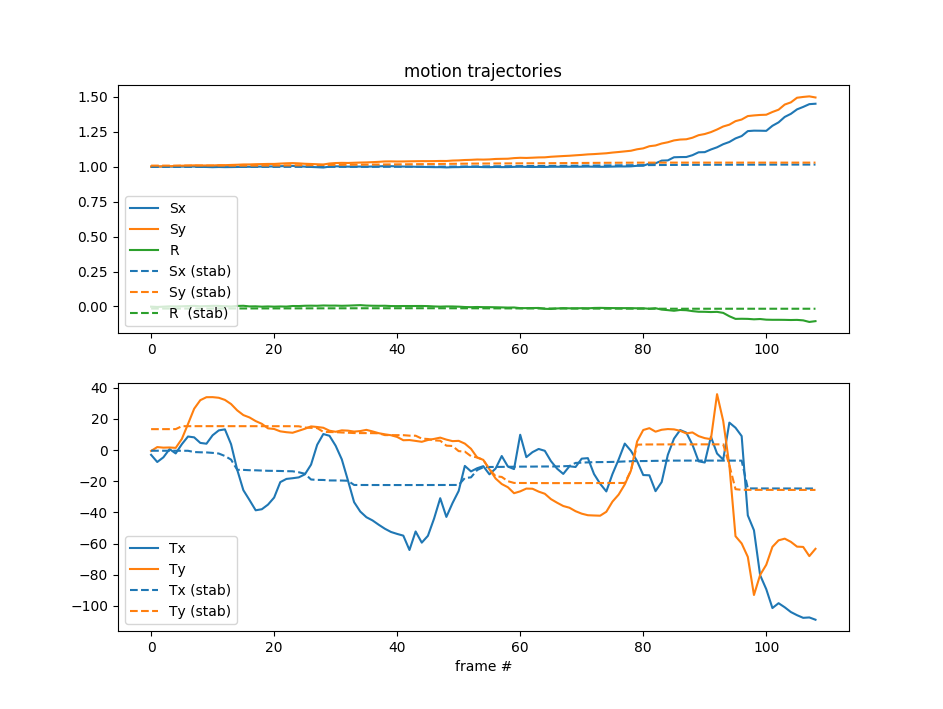
\includegraphics[width=0.9\textwidth]{trajetory_FISTA3.png}
  \captionof{figure}{Original (solid) and optimized (dashed) camera motion. Only first order temporal motion differences are penalized.}
  \label{fig:trajFISTA3}
\end{center}
\begin{center}
  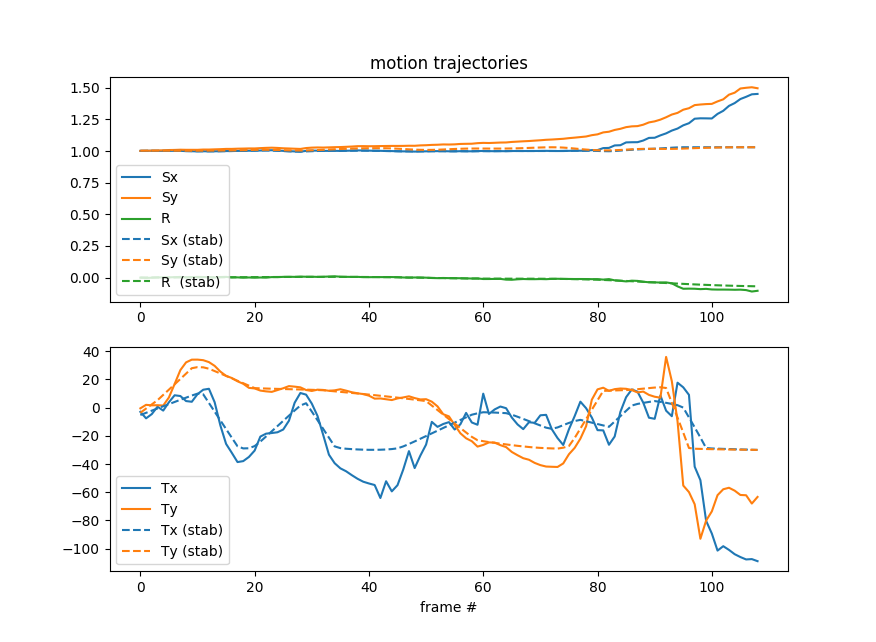
\includegraphics[width=0.9\textwidth]{trajetory_FISTA1.png}
  \captionof{figure}{Original (solid) and optimized (dashed) camera motion. Only second order temporal motion differences are penalized.}
  \label{fig:trajFISTA1}
\end{center}
\begin{center}
  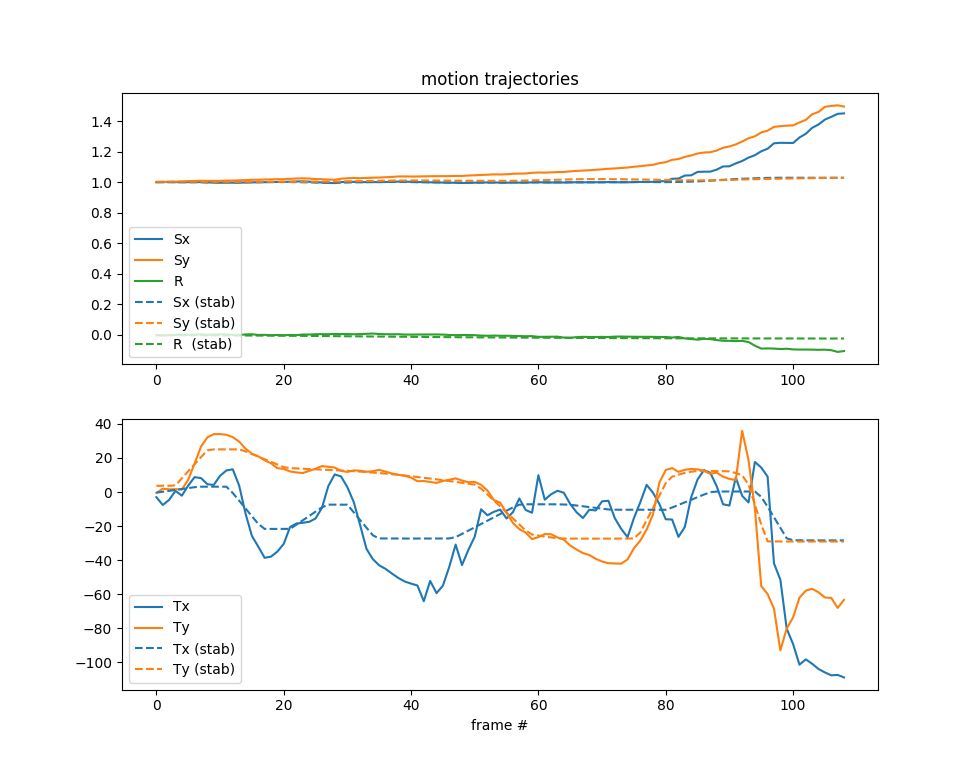
\includegraphics[width=0.9\textwidth]{trajetory_FISTA2.png}
  \captionof{figure}{Original (solid) and optimized (dashed) camera motion. Both first and second order temporal motion differences are penalized.}
  \label{fig:trajFISTA2}
\end{center}

\section{Conclusions}
The formalism used to achieve for video stabilization in this work has been designed to make use of large-scale first order optimization methods, such as FISTA. Using an objective function that penalizes both deviations from the original camera motion trajectory and abrupt changes in both the camera position and 1st order derivatives, stabilized footage is obtainable that emulates many of the qualities of professional video capture, most commonly restricted to high-budget productions. It is worth noting that although the formulation of the minimization problem in (\ref{eq:optprob2}) can be solved efficiently for large $N$ (number of video frames), the use of iterative optimization techniques is still too slow to permit use in online stabilization, where the time allotted to motion correction is often less than 42ms (at 24fps) or even 16ms (at 60fps). It is also worth noting that there are other interesting implementations of offline optimization-based video stabilization methods that add additional constraints for limiting the amount of frame cropping required after motion correction, in-painting the missing border information, and maintaining a full view of an interesting subset of the salient points (such as those of a human face). There are many other interesting opportunities for extending this work, and there shouldn't be any shortage of interest in this topic in coming years as computational photography and videography techniques continue to unlock new potential in what is possible from low-cost and highly available recording equipment.

\bibliography{report}
\bibliographystyle{iclr2019_conference}

\end{document}
